\section{Approach}
\label{sec:approach}
\OurApproach{}, our KGQA approach, consists of two phases: (1) question interpretation, and (2) answer inference.
In the question interpretation phase we identify the sets of entities and predicates that we consider relevant for answering the input question along with the corresponding confidence scores.
In the second phase these confidence scores are propagated and aggregated directly over the structure of the KG, to provide a confidence distribution over the set of possible answers.
Our notion of KG is inspired by common concepts from the Resource Description Framework (RDF)~\cite{rdf-primer}, a standard representation used in many large-scale knowledge graphs, e.g., DBpedia and Wikidata:

\begin{definition}
\label{def:kg}
\rm
We define a (knowledge) \emph{graph} $K=\langle E,G,P\rangle$ as a tuple that contains sets of \emph{entities} $E$ (nodes) and \emph{properties} $P$, both represented by Unique Resource Identifiers (URIs), and a set of directed labeled edges $\langle e_i, p, e_j\rangle\in G$, where $e_i, e_j \in E$ and $p \in P$.
\end{definition}

\noindent%
The set of edges $G$ in a KG can be viewed as a (blank-node-free) RDF graph, with subject-predicate-object triples $\langle e_i, p, e_j\rangle$.
In analogy with RDFS, we refer to a subset of entities $C \subseteq E$ appearing as objects of the special property \texttt{\small rdf:type} as \emph{Classes}.
We also refer to classes, entities and properties collectively as \textit{terms}.
We ignore RDF literals, except for \texttt{\small rdfs:labels} that are used for matching questions to terms in KG.

The task of \emph{question answering over a knowledge graph} (KGQA) is: given a natural language question $Q$ and a knowledge graph $K$, produce the correct answer $A$, which is either a subset of entities in the KG $A \subseteq E$ or a result of a computation performed on this subset, such as the number of entities in this subset (\smalltt{COUNT}) or an assertion (\smalltt{ASK}).
These types of questions are the most frequent in existing KGQA benchmarks~\cite{DBLP:journals/corr/BordesUCW15,DBLP:conf/semweb/TrivediMDL17,DBLP:conf/semweb/UsbeckGN018}.
In the first phase \OurApproach{} maps a natural language question $Q$ to a structured model $q$, which the answer inference algorithm will operate on then. 

\subsection{Question interpretation}

To produce a question model $q$ we follow two steps: (1) \textit{parse}, which extracts references (entity, predicate and class mentions) from the natural language question and identifies the question type; and (2) \textit{match}, which assigns each of the extracted references to a ranked list of candidate entities, predicates and classes in the KG.

Effectively, a complex question requires answering several sub-questions, which may depend on or support each other. A dependence relation between the sub-questions means that an answer $A^1$ to one of the questions is required to produce the answer $A^2$ for the other question: $A^2=f(A^1,K)$. 
We call such complex questions \textit{compound} questions and match the sequence in which these questions should be answered to \textit{hops} (in the context of this paper, one-variable graph patterns) in the KG.
Consider the sample compound question in Fig.~\ref{fig:qi}, which consists of two hops: (1) find the car types assembled in Broadmeadows Victoria, which have a hardtop style, (2) find the company, which produces these car types. There is an intermediate answer (the car types with the specified properties), which is required to arrive at the final answer (the company).

Accordingly, we define (compound) questions as follows:

\begin{definition}\label{def:question}
\rm
A \emph{question model} is a tuple $q=\langle t_q, Seq_q \rangle$, where $t_q \in T$ is a question type required to answer the question $Q$, and $Seq_q = (\langle E^i, P^i, C^i\rangle)_{i=1}^h$ is a sequence of $h$ hops over the KG, $E^i$ is a set of entity references, $P^i$ -- a set of property references, $C^i$ -- a set of class references relevant for the \textit{i}-hop in the graph, and $T$ -- a set of question types, such as $\{\smalltt{SELECT}, \smalltt{ASK}, \smalltt{COUNT}\}$.
\end{definition}

\noindent%
Hence, the question in Fig.~\ref{fig:qi} can be modeled as: $\langle \smalltt{SELECT}, (\langle E^1={}$\{``hardtop'', ``Broadmeadows, Victoria''\}, $P^1={}$\{``assembles'', ``style''\}, $C^1={}$\{``cars''\}$\rangle, \langle E^2=\emptyset, P^2={}$\{``company''\}, $C^2=\emptyset\rangle) \rangle$, where $E^i$, $P^i$, $C^i$ refer to the entities, predicates and classes in hop $i$.

Further, we describe how the question model $q$ is produced by parsing the input question $Q$, after which we match references in $q$ to entities and predicates in the graph $K$.

\OurParagraph{Parsing.}
Given a natural language question $Q$, the goal is to classify its type $t_q$ and parse it into a sequence $Seq_q$ of reference sets according to Definition~\ref{def:question}.
Question type detection is implemented as a supervised classification model trained on a dataset of annotated question-type pairs that learns to assign an input question to one of the predefined %question 
types $t_q \in T$.

We model reference (mention) extraction $Seq_q$ as a sequence labeling task~\cite{DBLP:conf/icml/LaffertyMP01}, in which a question is represented as a sequence of tokens (words or characters).
Then, a supervised machine learning model is trained on an annotated dataset to assign labels to tokens, which we use to extract references to entities, predicates and classes.
Moreover, we define the set of labels to group entities, properties and classes referenced in the question into $h$ hops.

\begin{figure*}[!t]
\centering
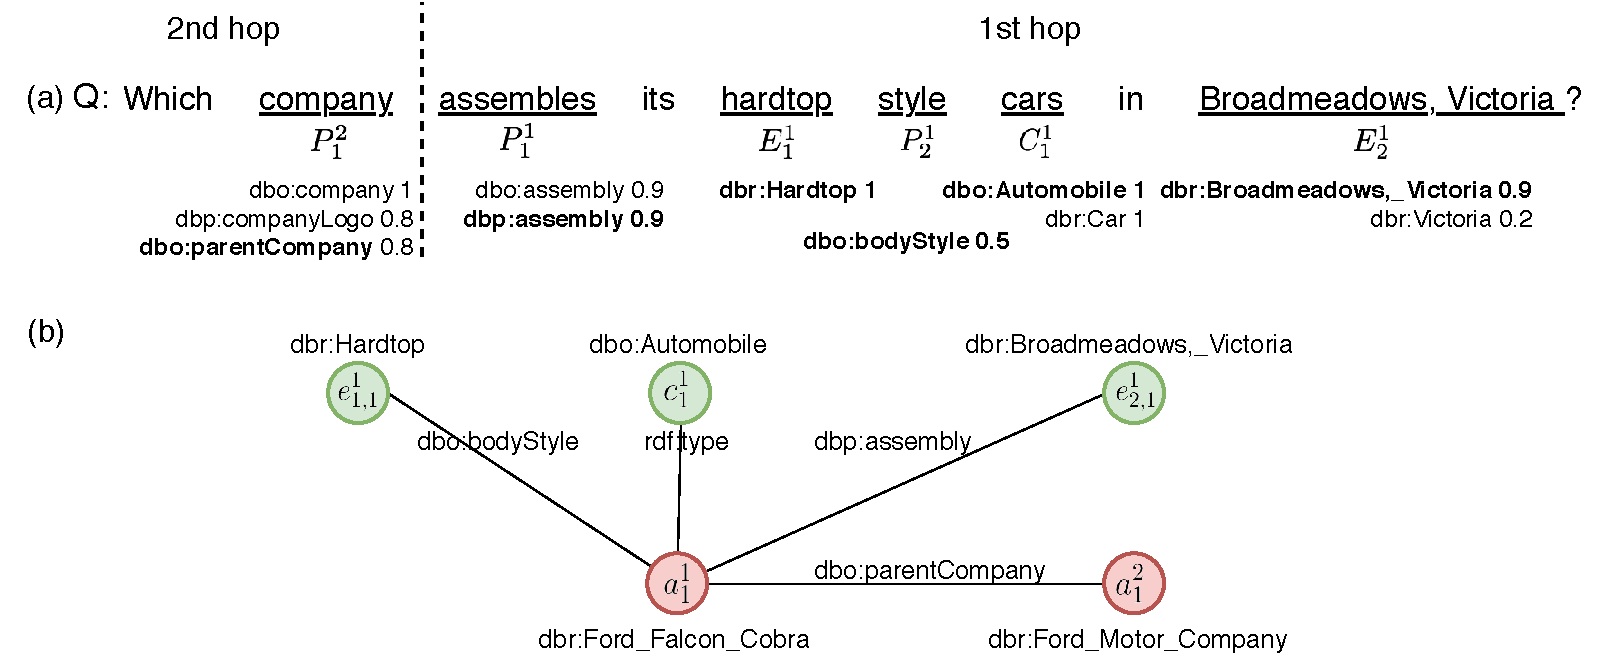
\includegraphics[width=0.9\textwidth]{figs/mp_example_linking.pdf}
\caption{(a) A sample question $Q$ highlighting different components of the question interpretation model: references and matched URIs with the corresponding confidence scores, along with (b) the illustration of a sample KG subgraph relevant to this question. The URIs in bold are the correct matches corresponding to the KG subgraph.}
\label{fig:qi}
\end{figure*}

\OurParagraph{Matching.}
Next, the question model (Definition~\ref{def:question}) is updated with an \emph{interpreted question model} $I(q) = (t_q, SEQ_q)$
%\todo[inline]{MC Check whether the following is correct}
%Here $SEQ_q$ has an entry for each step in $Seq_q$, containing possible matches in the knowledge graph and an assigned confidence.
%Each entry is a triple $\langle E^i, P^i, C^i \rangle$, where $X_i$ is a set of tuples which 
in which each component of $Seq_q$ is represented by sets of pairs from $(E \cup P \cup C) \times [0, 1]$ obtained by matching the references to concrete terms in $K$ (by their URIs) as follows: for each entity (or property, class, resp.) reference in $Seq_q$, we retrieve a ranked list of most similar entities from the KG along with the matching confidence score.

Fig.~\ref{fig:qi} also shows the result of this matching step on our example.
For instance, the property references for the first hop are replaced by the set of candidate URIs: $P^1 = \{P_1^1, P_2^1 \} \in SEQ_q$ within $I(q)$, where $P_1^1 = \{ \texttt{(\small  dbo:assembly}, 0.9)$, $(\texttt{\small dbp:assembly}, 0.9)\}$, $P_2^1 = \{ (\texttt{\small dbo:bodyStyle}, 0.5)\}$.
